%%%%%%%%
\subsection{Redes Neuronales Convolucionales (CNN)}


Las Redes Neuronales Convolucionales (CNN, por sus siglas en inglés) son una clase de modelos de aprendizaje profundo ampliamente utilizadas en tareas de visión por computadora, como clasificación de imágenes, detección de objetos y segmentación semántica. Su arquitectura está diseñada para capturar patrones espaciales jerárquicos en las imágenes mediante la aplicación de filtros convolucionales que extraen características locales. \parencite{lecun1998gradient}

Una CNN típica se compone de capas convolucionales, funciones de activación no lineales como ReLU, capas de normalización, y capas de pooling que reducen la dimensionalidad espacial, manteniendo la información más relevante. Las características extraídas en capas tempranas tienden a ser más simples (como bordes o texturas), mientras que las capas más profundas capturan patrones de alto nivel (como estructuras faciales o patrones morfológicos) \parencite{krizhevsky2012imagenet}

En el contexto de segmentación de imágenes de piel facial, las CNN permiten detectar y delimitar con precisión características morfológicas como arrugas, poros y manchas, debido a su capacidad de aprendizaje automático basado en ejemplos etiquetados. Además, su arquitectura se adapta fácilmente a modelos más complejos, como U-Net y DeepLabV3+, que han demostrado alto rendimiento en segmentación biomédica y estética. \parencite{ronneberger2015unet}

%\subsubsection{Ventajas y Limitaciones}  
%Las CNN ofrecen varias ventajas, entre ellas:
%\begin{itemize}
%    \item Alta precisión en la extracción y análisis de características complejas.
%    \item Automatización de procesos que tradicionalmente dependen de evaluaciones subjetivas.
%    \item Adaptabilidad a diferentes tipos de imágenes y tareas específicas.
%\end{itemize}

%Sin embargo, estas redes también presentan desafíos, como la necesidad de grandes volúmenes de datos etiquetados para el entrenamiento, el alto costo computacional y la posibilidad de sobreajuste si no se implementan técnicas adecuadas de regularización.

%En el presente estudio, las CNN se utilizarán para desarrollar un sistema avanzado de segmentación de imágenes faciales, optimizado para la detección de arrugas, poros y manchas. Este enfoque busca contribuir al sector cosmético y de belleza, permitiendo una evaluación estética más precisa y la personalización de tratamientos cosméticos.

%%%%%%%%%%%%%%%%%%%%%%%%%%%%%%%%%%%%%%%%%%%%%%%%%%%%%%%%%%%%%%%%%%%%%%
\subsection{Segmentación de Imágenes}
La segmentación de imágenes es el proceso de dividir una imagen en diferentes partes o regiones, con el objetivo de simplificar la representación de la imagen y hacerla más significativa y fácil de analizar. Este proceso es fundamental en aplicaciones de visión por computadora, especialmente en la detección de características morfológicas de la piel, como arrugas, poros y manchas \parencite{autor2020segmentacion}.
%%%%%%%%%%%%%%%%%%%%%%%%%%%%%%%%%%%%%%%%%%%%%%%%%%%%%%%%%%%%%%%%%%%%%%

\subsection{Características Morfológicas del rostro}
Las características morfológicas de la piel desempeñan un papel crucial en la evaluación de la salud y la estética facial, ya que ofrecen información valiosa sobre el estado general de la piel y sus posibles alteraciones. En este estudio, se consideran tres características clave: arrugas y manchas. La correcta segmentación de estas características en imágenes faciales permite no solo el análisis cuantitativo de las mismas, sino también su monitoreo a lo largo del tiempo, contribuyendo al diseño de tratamientos cosméticos personalizados y a la evaluación de su efectividad. \parencite{autor2021arrugas}

\subsubsection{Arrugas}
Las arrugas son pliegues o líneas visibles en la superficie de la piel que se forman debido a la disminución de la elasticidad y el colágeno con el envejecimiento. Factores externos, como la exposición prolongada al sol, la contaminación y el tabaquismo, también contribuyen significativamente a su aparición. Además, las expresiones faciales repetitivas y la deshidratación de la piel pueden acelerar su desarrollo. \parencite{autor2021arrugas}

Desde el punto de vista estético, las arrugas se asocian con el envejecimiento y son una de las principales preocupaciones en el cuidado de la piel. Su segmentación precisa permite identificar su profundidad, longitud y densidad en diferentes áreas del rostro. Esta información es esencial para el desarrollo de productos antiarrugas y para evaluar la efectividad de tratamientos como cremas tópicas, terapias con láser o inyecciones de ácido hialurónico. \parencite{autor2021arrugas}

\subsubsection{Manchas}
Las manchas son áreas de hiperpigmentación o hipopigmentación en la piel que resultan de una variedad de factores, incluyendo la exposición solar prolongada, cambios hormonales, envejecimiento y procesos inflamatorios. Ejemplos comunes incluyen el melasma, las manchas solares y las cicatrices post-inflamatorias. \parencite{autor2019manchas}

Estas imperfecciones no solo afectan la apariencia de la piel, sino que también pueden indicar daño subyacente. Por ello, su detección y análisis temprano son fundamentales tanto para la prevención como para el tratamiento. La segmentación precisa de manchas en imágenes faciales permite identificar su forma, tamaño, color y evolución, lo que es útil para personalizar tratamientos como cremas despigmentantes, terapias con luz pulsada intensa (IPL) o procedimientos láser. Además, este análisis contribuye al diseño de cosméticos específicos que ayudan a unificar el tono de la piel. \parencite{autor2019manchas}
%%%%%%%%%%
\subsubsection{Aplicaciones en Segmentación de Imágenes Faciales}  
En el ámbito del análisis de piel facial, las CNN son una herramienta fundamental para realizar segmentaciones precisas de características morfológicas, como arrugas y manchas. Gracias a su capacidad para analizar imágenes a nivel de píxel, estas redes son capaces de identificar patrones y diferencias en la textura, el color y la estructura de la piel. \parencite{autor2021deeplab}

\paragraph{Segmentación de arrugas}  
La segmentación de arrugas mediante CNN permite identificar líneas finas y pliegues en la piel, lo que es crucial para evaluar el envejecimiento facial y desarrollar tratamientos preventivos o correctivos. Este análisis automatizado es más preciso y rápido en comparación con las evaluaciones manuales, que pueden ser subjetivas y menos consistentes. \parencite{autor2020segmentacion}

%\paragraph{Detección de poros.}  
%La identificación y segmentación de poros faciales es esencial para analizar problemas relacionados con la textura de la piel, como poros dilatados o acné. Las CNN pueden cuantificar el tamaño, la densidad y la distribución de los poros, facilitando la personalización de tratamientos según las necesidades específicas de cada individuo.

\paragraph{Segmentación de manchas}  
Las manchas faciales, que pueden surgir debido a factores como la exposición solar o el envejecimiento, son una preocupación estética común. Las CNN permiten mapear su distribución y evaluar su progresión, ayudando a diagnosticar problemas como el melasma o el daño solar de manera temprana y objetiva. \parencite{autor2020segmentacion}


%%%%%%%%%%%%%%%%%%%%%%%%%%%%%%%%%%%%%%%%%%%%%%%%%%%%%%%%%%%%%%%%%%%%%%
%\subsection{Procesamiento en Tiempo Real}


%%%%%%%%%%%%%%%%%%%%%%%%%%%%%%%%%%%%%%%%%%%%%%%%%%%%%%%%%%%%%%%%%%%%%%
\subsection{Modelos de Segmentación Utilizados}

Para el desarrollo del sistema de segmentación de características morfológicas en imágenes de piel facial, se han seleccionado modelos basados en redes neuronales convolucionales (CNN) y arquitecturas híbridas con mecanismos de atención. Estos modelos han demostrado un rendimiento destacado en tareas de segmentación semántica, especialmente en aplicaciones biomédicas y de visión por computadora. A continuación, se describen brevemente los modelos que serán considerados:

\begin{itemize}
    \item \textbf{U-Net:} Es una arquitectura ampliamente utilizada en segmentación de imágenes médicas. Su diseño encoder-decoder con conexiones tipo \textit{skip} permite preservar detalles espaciales relevantes mientras se capturan características de alto nivel. \parencite{ronneberger2015unet}

    \item \textbf{Attention U-Net:} Extiende la arquitectura original de U-Net integrando mecanismos de atención, los cuales permiten al modelo enfocarse en las regiones morfológicamente más relevantes de la imagen. \parencite{oktay2018attentionunet}

    \item \textbf{DeepLabV3+:} Utiliza convoluciones dilatadas y un módulo de agrupación espacial piramidal (ASPP) para capturar información contextual a múltiples escalas. \parencite{chen2018deeplabv3plus}

    \item \textbf{BiSeNet v2:} Diseñado para segmentación en tiempo real, combina una rama detallada para preservar la resolución con una rama contextual que extrae características globales. \parencite{yu2021bisenetv2}

    \item \textbf{UNETR:} Integra bloques de Transformer dentro de la arquitectura tipo U-Net para modelar dependencias espaciales de largo alcance. Ha sido evaluado con éxito en imágenes médicas volumétricas y ofrece un alto rendimiento en segmentación precisa. \parencite{hatamizadeh2022unetr}
\end{itemize}

La inclusión de estos modelos permitirá realizar un análisis comparativo para identificar cuál ofrece el mejor rendimiento en la segmentación de características morfológicas faciales como arrugas, poros y manchas, especialmente en escenarios de procesamiento en tiempo real.
%%%%%%%%%%%%%%%%%%%%%%%%%%%%%%%%%%%%%%%%%%%%%%%%%%%%%%%%%%%%%%%%%%%%%%

%%%%%%%%%%%%%%%%%%%%%%%%%%%%%%%%%%%%%%%%%%%%%%%%%%%%%%%%%%%%%%%%%%%%%%
%\subsection{Metricas de Evaluación}

%%
%%%%%%%%%%

%%%





\begin{comment}

\subsection{Ecografía y las imágenes de ultrasonido}
Según \cite{pr_herrera2017diseimp}, la ecografía, que es una técnica de diagnóstico en donde se usan imágenes generadas por ultrasonido, es comúnmente desarrollado en las áreas de cardiología, ginecología, y otras más relacionadas. La popularidad de esta técnica se basa en la capacidad de las imágenes de alta calidad que se obtienen de este proceso, además de no ser un método invasivo o de radiación como muchos otros de su tipo.

Los sistema encargados de extraer las imágenes de ultrasonido son compuestos de distintas sensores que generan ondas de sonido para posteriormente analizar la respuesta de la interacción física con el campo de interés. Estas señales recibidas de regreso son digitalizados por una parte electrónica delantera que también transforman estos datos crudos en la imagen final. El funcionamiento de este proceso depende de la configuración de los sensores, el método usado para obtener las imágenes y las características de área de interés. \parencite{pr_camacho2022ultrasonicimg}

Algunas imágenes de ultrasonido de nódulos tiroideos se muestran en la Figura \ref{2:fig210}.

\begin{figure}[H]
	\begin{center}
		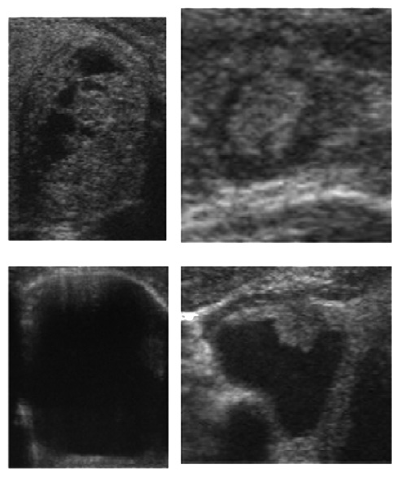
\includegraphics[width=0.40\textwidth]{2/figures/imagenes_ultrasonido_originales.png}
		\caption[Imágenes de ultrasonido de nódulos tiroideos]{Imágenes de ultrasonido de nódulos tiroideos. \\
		Fuente: \cite{pr_JERBI2023autoclassViTGAN}. \textit{Automatic classification of ultrasound thyroids images using vision transformers and generative adversarial networks}.}
		\label{2:fig210}
	\end{center}
\end{figure}


\subsection{Transfer Learning}
\cite{bk_geron2022handml} nos menciona que el Transfer Learning o Transferencia de Aprendizaje es un técnica usada en el campo de Deep Learning que permite el uso de algunas capas de un modelo ya definido y entrenado previamente en un nuevo modelo que necesite ser entrenado en una tarea similar al que se desarrolla el modelo original. Las capas destinadas al reuso son normalmente las más cercanas a la entrada o también conocidas como capas inferiores. El beneficio de usar esta técnica radica en dos puntos importantes: cantidad de datos requeridos y velocidad de entrenamiento del modelo; es decir, la cantidad de datos que se deben usar para entrenar un modelo de alto desempeño se reduce considerablemente, mientras que el tiempo requerido para terminar este proceso es menor comparándolo a si lo entrenaran desde cero.

Para que esta técnica funcione debidamente, las capas más cercanas a la salida, conocidas también como capas de alto nivel, deben ser reemplazadas, esto debido a que son más específicas de las tareas del modelo original. Esto también incluye a la capa final, ya que posiblemente no tenga la cantidad de salidas necesarias para completar satisfactoriamente la nueva tarea.

En la Figura \ref{2:fig211} se presenta de forma gráfica la técnica.

\begin{figure}[H]
	\begin{center}
		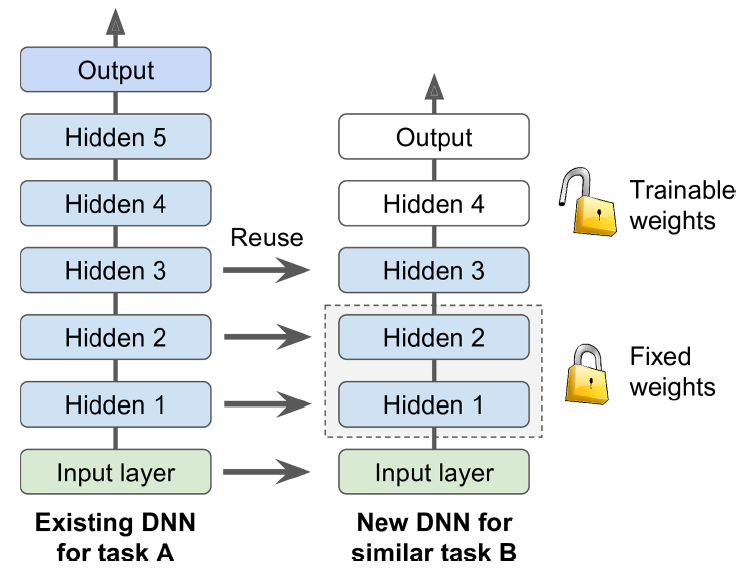
\includegraphics[width=0.70\textwidth]{2/figures/transfer_learning.PNG}
		\caption[Ejemplo de Transfer Learning]{Ejemplo de Transfer Learning. \\
		Fuente: \cite{bk_geron2022handml}. \textit{Hands-on machine learning with Scikit-Learn, Keras, and TensorFlow}.}
		\label{2:fig211}
	\end{center}
\end{figure}


\subsection{Data Augmentation}

Según \cite{bk_geron2022handml} el Aumento de Datos o Data Augmentation es una técnica de regularización que permite reforzar la cantidad de muestras en un conjunto de datos. Esto se realiza a través de la generación de nuevas instancias similares a los originales; es decir, las personas no deberían ser capaces de diferenciar una imagen generada de una del propio conjunto de datos.

Para generar estas nuevas muestras, normalmente se aplican diferentes transformaciones a las instancias del conjunto de datos original. Estas transformaciones pueden ser; por ejemplo, una simple rotación o recorte de la imagen, siempre y cuando no altere por completo su sentido como es el caso de voltear una imagen de texto de forma horizontal. 

El principal beneficio de esta técnica es que permite reducir el sobreajuste de los modelos entrenados. 

En la Figura \ref{2:fig212} se muestran algunas transformaciones que se pueden hacer al aplicar el Aumento de Datos. 

\begin{figure}[H]
	\begin{center}
		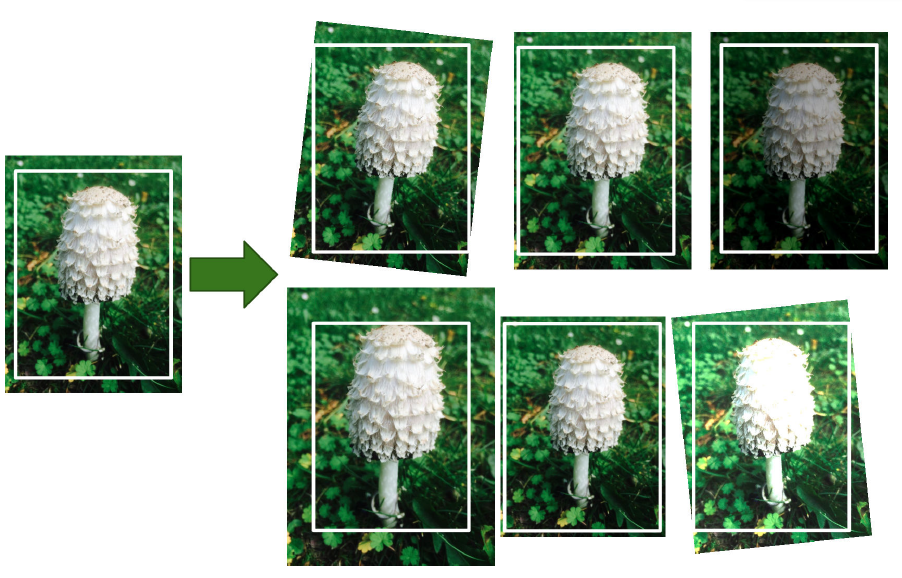
\includegraphics[width=0.85\textwidth]{2/figures/data_aug.PNG}
		\caption[Ejemplo de Data Augmentation]{Ejemplo de Data Augmentation. \\
		Fuente: \cite{bk_geron2022handml}. \textit{Hands-on machine learning with Scikit-Learn, Keras, and TensorFlow}.}
		\label{2:fig212}
	\end{center}
\end{figure}

\end{comment}